Finora abbiamo visto reazioni chimiche che generano energia elettrica. Facciamo il contrario: prendiamoo una soluzione, immergiamo due elettrodi e applichiamo una d.d.p. dall'esterno.

Ciò che stiamo facendo è l'opposto di ciò che viene nelle pile. In esse infatti sfruttiamo reazioni chimiche per generare energia eletrrica, qui invece imponismo una una d.d.p. esterna e vogliamo vedere se avvengono reazioni chimiche. Tali reazioni dovranno avvenire, perché se avessimo sull'elettrodo e elettroni e ioni positivi in soluzione, quest'ultimi tenderanno a depositarsi sull'elettrodo, catturando gli elettroni e quindi riducendosi. Se però su un elettrodo si ha riduzione, sull'altro dovrà avvenire un'ossidazione perché il circuito deve essere chiuso, altrimenti non fluirebbero gli elettroni da un elettrodo all'altro.

Consideriamo allora una soluzione di HCl in cui immergiamo due fili di platino e applichiamo una piccola d.d.p. che va via via aumentando. Man mano che sale riportiamo su un grafico i valori di intensità di corrente misurata e la d.d.p. appicata dall'esterno. Ci si accorge che se abbiamo un filo metallico, all'aumentare della d.d.p. aumenta anche la corrente che passa sul filo, mentre se abbiamo una soluzione ciò non accade.

Se adoperiamo un amperometro avente prontezza elavata, il quale misura immediatamente le più piccole variazioni di corrente, ci accorgiamo che la corrente ha un picco e poi ritorno a zero. Man mano che la d.d.p. aumenta avremo diversi picchi, fin quando questa non raggiunge un certo valore. Se invece non avessimo uno strumento abbastanza pronto vedremmo una corrente di fondo che poi invece cresce bruscamente:

\begin{figure}[H]
    \centering
    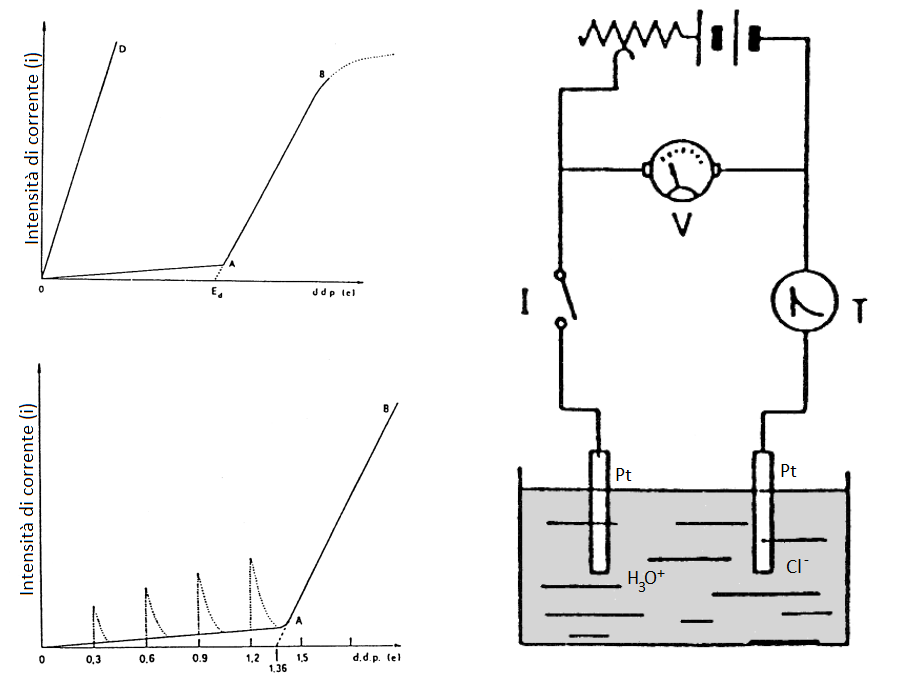
\includegraphics[width=14cm]{immagini/elettrolisi.png}
\end{figure}

A cosa è dovuto questo fenomeno?

In soluzione abbiamo HCl. Stiamo mettendo due fili di platino, che è un metallo nobile, inerte. Se applichiamo una d.d.p. ci aspettiamo che lo ione $\rm H_3O^+$ acquisti due elettroni e diventi $\rm H_2$, cioè si riduca, e questi due elettroni vengono forniti da due ioni $\rm Cl^-$
\subsection{Leggi di Faraday}
Il fenomeno dell'elettrolisi è generato dalle due leggi di Faraday

\vspace{0.2cm}$\bullet$\textbf{Prima legge di Faraday}

\vspace{0.2cm}$\bullet$\textbf{Prima legge di Faraday}

\subsection{Accumulatore al piombo (batteria automobile)}

\begin{figure}[H]
    \centering
    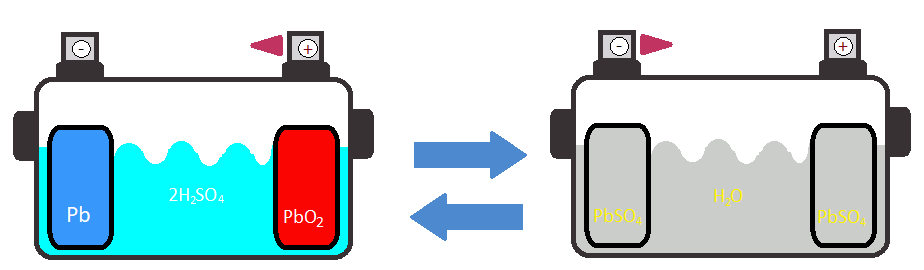
\includegraphics[width=15cm]{immagini/accumulatore_al_piombo.png}
\end{figure}

Abbiamo l'anodo costituito da piombo metallico e il catodo da $\rm PbO_4$ (quindi $\rm Pb^{4+}$). La soluzione che ci permette di trasportare gli elettrodi è acido solforico $\rm H_2SO_4$ molto concentrato, al 30\%, tant'è che quando si abbassa il livello del liquido nella batteria non si aggiunge acido ma acqua, in quanto l'$\rm H_2SO_4$ bolle a 400° C, per cui se il livello si è abbassato sarà evaporata soltanto l'acqua.

Quando si carica ciò che succede è che il $\rm Pb^0(s)$ in presenza di acido solforico (e quindi di ioni solfato $SO_4^{2-}$) libera 2 elettroni, diventando $\rm Pb^{2+}$. Si unisce quindi allo ione solfato dando $\rm PbSO_4$ e liberando 2 elettroni.

$$(-)\; \ce{Pb(s) + SO_4^{2-} -> PbSO_4(s) + 2e^-}$$

Questi due elettroni vengono catturati dal $\rm PbO_2(s)$, e il piombo passa da $\rm Pb^{4+}$ a $\rm Pb^{2+}$, per poi unirsi allo ione solfato e diventare $\rm PbSO_4$:

$$(+)\; \ce{PbO_2(s) + 4H_3O^+ + SO_4^{2-} +2e^- -> PbSO_4(s) + 6H_2O}$$

Quindi in entrambi i casi si forma $\rm PbSO_4$, però una volta a partire da $\rm Pb^0$ che deve liberare 2 elettroni e una volta a partire da $\rm Pb^{4+}$ che deve acquistare 2 elettroni.

Nel proceso di carica invece avviene l'opposto: abbiamo $\rm PbSO_4$ (quindi $\rm Pb^{2+}$) che nell'anodo assorbe 2 elettroni diventando Pb(s) mentre nel catodo cede 2 elettroni diventando $\rm Pb^{4+}$:

$$(-) \; \ce{PbSO_4(s) + 2e^- -> Pb(s) + SO_4^{2-}}$$

$$(+) \; \ce{PbSO_4(s) + 6H_2O  -> PbO_2(s) + 4H_3O^+ + SO_4^{2-} +2e^-}$$